% Preamble ==================================================================
\documentclass[11pt]{article}
\usepackage{geometry}
\geometry{verbose,tmargin=2.5cm,bmargin=2.5cm,lmargin=2.5cm,rmargin=2.5cm}
\usepackage{float}
\usepackage{graphicx} %for pictures and graphics

\usepackage{color}
\usepackage{amsmath}
\usepackage{amssymb}
\usepackage{mathtools}
\usepackage{fixltx2e}
\usepackage{textcomp}
\usepackage{bibentry}

\usepackage[ labelsep=period, justification=raggedright, margin=10pt,font={small},labelfont={small,normal,bf,sf}]{caption}


%----------------------
%Reduce spacing above title
\usepackage{titling}
\setlength{\droptitle}{-5em}
\posttitle{\par\end{center}\vspace{-1pt}} %Use if don't have an author

%----------------------------------------------------
%Format section heading style
\usepackage{sectsty}
\sectionfont{\sffamily\bfseries\small}
\subsectionfont{\sffamily\small\slshape}
\subsubsectionfont{\sffamily\small\itshape}


%Put period after section number
\makeatletter
\def\@seccntformat#1{\csname the#1\endcsname.\quad}
\makeatother


\renewcommand\familydefault{\sfdefault}

\setlength{\parskip}{0ex} %No space between paragraphs.

%PUT ME LAST--------------------------------------------------
\usepackage[colorlinks=true
,urlcolor=black
,anchorcolor=black
,citecolor=black
,filecolor=black
,linkcolor=black
,menucolor=black
,linktocpage=true
,pdfproducer=medialab
,pdfa=true
,hypertexnames=false
]{hyperref}

\makeatother 

%Preamble end================================================================



\begin{document}

\newcommand{\cotwo}{CO\textsubscript{2}}
\newcommand{\meth}{CH\textsubscript{4}}

\begin{flushleft}
\textsf{\textbf{\large{A Short, Quantitative, Summary of ``What Everyone Needs to Know about Climate Change''}}}
\end{flushleft}

\begin{flushleft}
\textsf{\textbf{Juvid Aryaman, Oct 2018}}
\end{flushleft}

\section{Introduction}



I am writing this document because it is difficult to find a concise synthesis of evidence supporting the claim that climate change poses (one of) the most important existential risk(s) to humanity. There also exists an abundance of disinformation on the topic, so it is important to find credible sources.

The evidence I have chosen to cite is largely based upon Joe Romm's recent book \cite{Romm18}. Ref.~\cite{Romm18} is a credible source of information on climate change because:
\begin{itemize}
\item Joe Romm is a credible expert.
\begin{itemize}
\item PhD in oceanography of the Greenland Sea from MIT, working with Walter Munk.
\item Worked for the U.S. Department of Energy as Acting Assistant Secretary for Energy Efficiency and Renewable Energy for 5 years.
\item Founder of Center for Energy and Climate Solutions, working with corporations to lower greenhouse gas emissions.
\item Founding editor of \url{ClimateProgress.org}.
\item In 2009, \textit{Time} magazine named him ``Hero of the Environment'' and ``The Web's most influential climate-change blogger''.
\item In 2016, Paul Krugman wrote in the \textit{New York Times} ``I've learnt a lot of what I know about energy economics from Joe Romm''.
\end{itemize}
\item Oxford University Press is a credible publisher.
\item Ref.~\cite{Romm18} is essentially an extended review article, and cites primary literature.
\item The references in Ref.~\cite{Romm18} are almost entirely from well-reputed scientific journals and reports, and are therefore relatively likely to reflect the consensus view of the scientific community.
\end{itemize}

Ref.~\cite{Romm18} is, however, 352 pages long, which presents a barrier to a layperson quickly understanding the importance of climate change. Generation of a set of quantitative claims, with corresponding citations, removes subjectivity from the discussion. There is therefore a need for a set of key, quantitative, claims to be made available which unambiguously state why climate change is of the utmost importance to humanity. 

Here, I will attempt to provide such a set of key, quantitative, claims. I will cite primary literature where it was obvious in Ref.~\cite{Romm18}. This document is an on-going effort, and suggestions for improvement are most welcome.  

\section{Contributors to climate change}

\subsection{Greenhouse gases}
\begin{itemize}
\item Satellite data show the Earth emitting less infrared radiation (comparing 1970 to 1997 levels) at the wavenumbers at which greenhouse gases such as \cotwo\ and \meth\ absorb energy \cite{Harries01}. This results in a significant increase in the amount of longwave downward radiation \cite{Philipona04}, which has been linked to various anthropogenic greenhouse gases \cite{Evans06}. These studies provide \textit{direct evidence} for the role of anthropogenic greenhouse gases in contributing to climate change (see \cite{SkepSci73}).
\item $>$90\% of all anthropogenic \cotwo\ comes from burning fossil fuels.
\item In 2012, \meth\ contributed up to 9\% of greenhouse gases. Major sources of \meth\ are: leaks in fossil fuel extraction, livestock, decaying organic waste, and some agricultural practices.
\item Brazil reduced its annual rate of Amazon deforestation by 80\% between 2004 and 2013. Deforestation is responsible for $\sim 8\%$ of all greenhouse gas emissions [Global Carbon Project].
\end{itemize}

\subsection{Permafrost}
\begin{itemize}
\item Permafrost is soil that stays below freezing for at least 2 years, sinking \cotwo\ from the carbon cycle. It locks up 1.7~trillion tonnes of carbon \cite{Tarnocai09}, which is twice of that in the atmosphere.
\item None of the IPCC's climate models include \cotwo\ or \meth\ emissions from permafrost as a feedback.
\item Anthropogenic \meth\ emissions are 0.5~bn tonnes per year, whereas the Siberian permafrost contains 70~bn tonnes. It is uncertain whether this carbon will be released as \meth\ or \cotwo. 
\item Assuming all permafrost emission as \cotwo, and IPCC scenario A1B \cite{IPCC07} (atmospheric \cotwo\ increases to
700 ppm by 2100, then stays constant at 700 ppm after 2100), permafrost carbon feedback is predicted to change the arctic from a carbon sink to a carbon source after the mid-2020's, and is strong enough to cancel 42-88\% of the total global land sink by 2100 \cite{Schaefer11} 
\item By 2100, permafrost could add 0.25\textdegree{}C, and possibly as much as 0.8\textdegree{}C \cite{Macdougall12}.
\end{itemize}

\subsection{Wildfires}
\begin{itemize}
\item The ``boreal'' (subarctic) forests rest on permafrost and peatland which release massive amounts of \cotwo\ when burned. They store $>30\%$ of all carbon stored on land. Boreal forests now have twice as many wildfires as 500-1000 years ago \cite{Kelly13}.
\item Peat is one of the earliest stages in the process of forming coal and burns easily. The peatland fires in Indonesia during 1997-1998 contributed 13-40\% of total \cotwo\ emissions for that year \cite{Page02}. Therefore peatland fires have a massive potential to contribute to carbon emissions.
\item When peatland dries out, wildfires become more severe \cite{Turetsky11}. Indonesia has drained a great deal of its peatlands, and burned forested areas, to create palm oil plantations.
\item Assuming the Amazonian dry season length (DSL) were to increase at half of the rates we observed during 1979--2011, the DSL would be about $1 \pm 1/3$~mo longer by 2090 than that in the 2000s \cite{Fu13}, potentially making the Amazon rainforest an important accelerating feedback for climate change \cite{Romm18}.
\end{itemize}

\subsection{Oceans}
\begin{itemize}
\item Ocean warming could cause a reduction in uptake of atmospheric \cotwo\ by 14--67 billion tonnes of carbon per year per \textdegree{}C of warming \cite{Gruber11}. Some models suggest this corresponds to as much as 30\% reduction in uptake by 2100, although most models suggest a more modest reduction \cite{Gruber11}.
\item As oceans acidify, phytoplankton appear to produce less dimethylsulphide, which plays a role in cloud formation, meaning more radiative forcing. This effect alone is estimated to contribute 0.23--0.48\textdegree{}C warming \cite{Six13}.
\end{itemize}

\section{\cotwo\ levels}
\begin{itemize}
\item \cotwo\ levels are curently at 400~ppm and rising at more than 2~ppm a year. Pre-industrial levels were 280~ppm (see Fig.~\ref{Fig:co2_history}).
\item \cotwo\ levels were approximately 440 ppm 15-20 million years ago, where the earth was 3-6\textdegree{}C warmer and sea levels 25-40~metres higher \cite{Tripati09}.
\item The last time \cotwo\ levels were comparable to today's levels was 3.6--2.2~million years ago (mid-Pliocene), where summer temperatures were approximately 8\textdegree{}C warmer than today, the WAIS did not exist, and sea levels were 25~metres higher than today \cite{Brigham13}.
\item Currently operating power generation infrastructure will commit us to 300 Gt\cotwo\ whereas the budget for a 1.5\textdegree{}C-2\textdegree{}C world is 240  Gt\cotwo\. Current pipeline power plants would add a further 270 Gt\cotwo. \cite{Pfeiffer18} 
\item Climate change that takes place due to increases in carbon dioxide concentration is largely irreversible for 1,000 years after emissions stop \cite{Solomon09}
\end{itemize}

\begin{figure}
\centerline{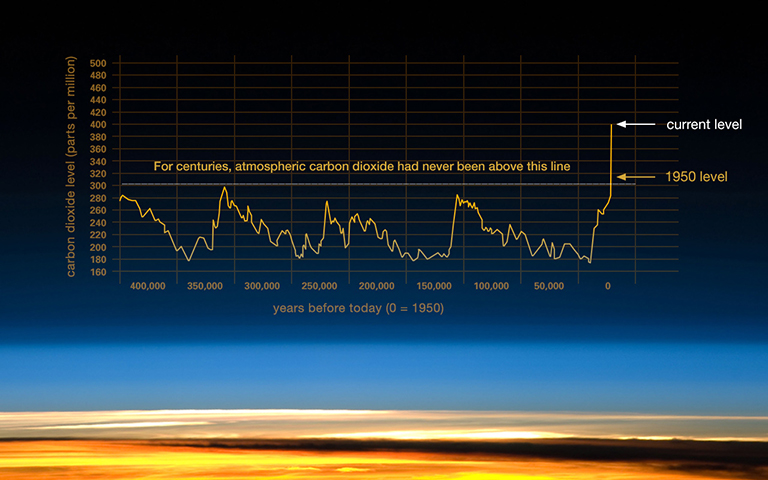
\includegraphics[width=0.8\columnwidth]{Figures/co2_nasa.jpg}}
\caption{\textbf{Human civilization has never seen \cotwo\ levels as high as they are today}. Image from Ref.~\cite{NasaCO2}.} 
\label{Fig:co2_history}
\end{figure}

\section{Temperature levels}
\begin{itemize}
\item If, as a whole, the planet warms by 4\textdegree{}C, much of the global population (which lives in the mid-latitudes: US and Europe) will face warming of 5 \textdegree{}C or more.
\end{itemize}


\section{Sea levels}
\begin{itemize}
\item If Greenland completely melts it will raise sea levels by $>$6 metres (20 ft).
\item If the Antarctic ice sheet completely melts it will raise sea levels by 60 metres (200 feet) [90\% of all Earth's ice].
\item The Antarctic ice sheet is losing 0.44 billion tonnes of ice per day (159 billion tonnes per year). \cite{Mcmillan14} 
\item One sector of the West Antarctic ice shelf (WAIS) seems to have passed a tipping point \cite{Rignot14}. The collapse of this sector would raise sea levels by 1.2~metres (4~ft) in the coming centuries. The sector acts as a linchpin for the stability of the WAIS.
\item The WAIS contains enough ice to induce 3.7--4.6 metres of sea level rise (12--15~ft).
\item Business as usual: 0.3~m (1~ft) rise by 2050, $>$1.2--1.8~m (4--6~ft) by 2100, rising 0.3~m per decade thereafter
\item Seas will likely rise by around 80~cm (2.6~ft), with the 95th percentile at 180~cm (5.9~ft) \cite{Jevrejeva14}.
\item A glacier in the East Antarctic Ice Sheet also appears to be highly unstable, and has the potential to raise sea levels by 3.5~m (11.5~ft) \cite{Greenbaum15}.
\item Antarctica has the potential to contribute more than 1~m (3.3~ft) of sea-level rise by 2100 \cite{Deconto16}
\item ``Recent findings have led top climatologists to conclude that we are likely headed toward what used to 3--5~ft of global sea level rise by 2100, with worst-case scenarios being much worse'' \cite{Romm18}
\item Between 315--411 million people may be living in the 100-year flood plain by 2060, compared to 189 million in the year 2000 \cite{Neumann15}. Subsidence in deltaic areas and from groundwater pumping could further enhance these numbers. Such storm-surges are expected to become far more common -- see Section~\ref{sec:flood_ss}.
\item Global mean sea level rise of 2.4~m (8~ft) by 2100 is physically possible, although the probability of such an outcome is hard to assess \cite{Wuebbles17}.
\item Projections of salinization in Bangladesh suggest that climate change will cause significant changes in river salinity, likely leading to shortages in drinking and irrigation water \cite{Dasgupta15}. This may reduce rice yields by $\sim$15\% \cite{Dasgupta14}.
\item If \cotwo\ peaks at 600~ppm, irreversible global average sea level rise of at least 0.4--1.0~m is predicted from thermal expansion alone \cite{Solomon09}.
\end{itemize}

\section{Heat waves, drought \& dustbowlification}
\begin{itemize}
\item In 2010, Russia suffered the most lethal heat wave in human history killing 55,000 people. Russia lost 40\% of its wheat crop, and banned grain exports for 18 months. These factors have been suggested to be implicated in the Syrian conflict \cite{Kelley15}.
\item The risk of a decade-scale megadrought in the U.S. southwest in the coming century is at least 80\%, and may be higher than 90\% in certain areas \cite{Ault14}
\item Severe and widespread droughts are predicted in the next 30--90 years over many land areas \cite{Dai13}, see Fig.~\ref{Fig:drought_Dai}. 
\item Drought conditions like the Dust Bowl of the 1930's are predicted to become normal in the U.S. Southwest and in other subtropical dry zones (reviewed in \cite{Seager07,Ault14}), see Fig.~\ref{Fig:drought_Dai} \cite{Dai13}.
\item Drought-affected areas are prediced to increase from 15.4\% of global cropland today, to around 44\% by 2100 \cite{Li09}.  The most severely affected regions in the next 30 to 90 years will likely be in southern Africa, the United States, southern Europe and Southeast Asia, says the report. In Africa, the report predicts 35\% of cropland will become unsuitable for cultivation in a 5\textdegree{}C world \cite{WB12}.
\item The growing season temperature at the end of the 21st century will likely exceed the hottest growing season ever observed in regions affecting half the world's population\cite{Battisti09}. 
\item Under a scenario where greenhouse gas emissions continue to grow, by 2100, $\sim$74\% of the Earth's population are forecast to be exposed to a mixture of mean surface air temperature and humidity that is deadly, for at least 20 days per year \cite{Mora17}. This is reduced to $\sim$48\% under a scenario of drastic greenhouse gas emissions, and is currently  $\sim$30\%.
\item Crop yields (mostly wheat, maize, rice, and soy) are forecast to likely reduce on the order of 10\% from around 2040 onwards, with $\sim$30\% of projections predicting a decrease in yield of $\sim$25\% or more by 2100 (Fig.~2.7, \cite{Allen14}). 
\end{itemize}

\begin{figure}
\centerline{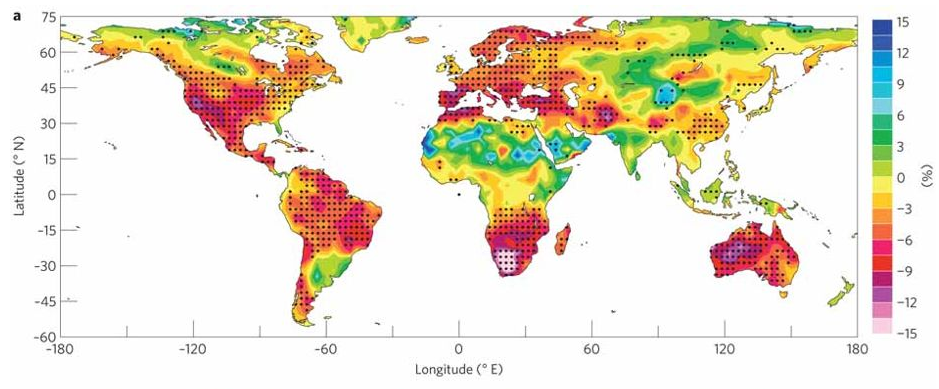
\includegraphics[width=\columnwidth]{Figures/Dai13_fig2a.png}}
\caption{\textbf{Severe and widespread droughts are predicted over the next century}. Percentage changes from 1980--1999 to 2080--2099 in the multimodel ensemble mean soil-moisture content in the top 10 cm layer under the RCP4.5 emissions scenario. Image from Ref.~\cite{Dai13} (Fig.~2a therein).} 
\label{Fig:drought_Dai}
\end{figure}

\section{Ocean acidification}
\begin{itemize}
\item Ocean acidification is causing many parts of the ocean to become undersaturated with calcium carbonate, which affects the ability of many oceanic organisms to form shells \cite{NOAA_ocean_acid} [CHECK SOURCE LATER].
\item Oceans are currently acidifying 10 times faster today than 55 million years ago when a mass extinction of marine species occurred \cite{Ridgwell10,Romm18}
\item Ocean acidification is irreversible on timescales of at least tens of thousands of years \cite{IAP09}.
\item Marine food supplies are likely to be reduced with significant implications for food production and security in regions dependent on fish protein \cite{IAP09}. The fish that grow and live on coral reefs are a significant food source for half a billion people worldwide \cite{Romm18}. 
\end{itemize}

\section{Costal flooding \& storm surges} \label{sec:flood_ss}
\begin{itemize}
\item 2-4 feet sea-level rise by 2100 results in hurricane Sandy-level storm surge events recurring about once per year or more across the US east-coast \cite{Sweet13}.
\item A 1\textdegree{}C rise in global temperature corresponds to 2--7 times increase in the frequency of Katrina magnitude storm surge events (which were 1 in 20 year events since 1923) \cite{Grinsted13}.
\end{itemize}



\section{Polar warming}
\begin{itemize}
\item Paleoclimate data shows that Arctic temperature change consistently exceeds the Northern Hemisphere average by a factor of 3-4 \cite{Miller10}.
\item The Arctic has warmed by 2\textdegree{}C since the 1970's \cite{Pistone14}. Over this period, the Arctic grew 8\% darker; the extra energy absorbed is equal to 25\% of the entire heat-trapping effect of \cotwo\ in that time \cite{Pistone14}.
\item 
\end{itemize}

\section{Economic impacts}
\begin{itemize}
\item Non-agricultural economic productivity reduces by 2.4\% per degree rise in temperature above 25\textdegree{}C\cite{Hsiang10}. 
\item Productivity impacts alone might reduce per capita output by $\sim$9\% in 2080-2099 (in the absence of strong adaptation).  This cost excedes the combined cost of all other projected economic losses combined \cite{Romm18,Hughes11} (see e.g.\  \cite{Stern06,Tol09}, which do not include temperature-related loss in productivity, and may underestimate economic costs by more than a factor of two).
\item \cotwo\ is a direct pollutant: at 930~ppm, six of nine decision-making performance domains were found to be impacted \cite{Allen15}. For most of human evolution and modern history, \cotwo\ levels in the atmosphere were between 180--280~ppm \cite{Romm18} (see Fig~\ref{Fig:co2_history}). Surveys of elementary schools in the US have reported \cotwo\ concentrations $>$1000~ppm in 45\% of 435 classrooms investigated, and was associated with student absence \cite{Corsi02,Allen15}. Peak \cotwo\ concentrations have been found to exceed 3000~ppm in 21\% of classrooms in a Texas survey \cite{Corsi02}.
\end{itemize}

\section{Biodiversity}
\begin{itemize}
\item There are very strong indications that the current rate of species extinctions far exceeds anything in the fossil record \cite{Magurran10}, being about 1000 times the background rate of extinction \cite{Pimm14}. 
\item By 2100, under business-as-usual projections, it is predicted that there will be a 50\% increase in the suboxic water volume ("dead zones"), in response to the respiration of excess organic carbon formed at higher \cotwo\ levels \cite{Oschlies08}. Intermittent periods of low oxygen levels resulting in marine suffocation have been recorded since 2002 \cite{Welch15}.
\end{itemize}

\section{Basic science}

\begin{itemize}
\item Global warming potential (GWP): Amount of heat trapped by a gas compared to the same mass of \cotwo, over a given period of time. 20 year GWP is more important due to the pressing nature of climate change, although 100 year GWP is more widely used.
\item \meth\ GWP = 34 over 100 years. \meth\ GWP = 86 over 20 years. 
\item If sea surface temperatures are below 26.5\textdegree{}C, tropical cyclones and hurricanes do not form
\item Polar amplification: where poles warm faster than the rest of the planet. This can weaken the jet stream, making weather last longer. 
\end{itemize}

\section{Further reading}
\begin{itemize}
\item \url{https://www.skepticalscience.com/}
\end{itemize}

\bibliographystyle{Bioessays}
\small{\bibliography{lit.bib}}

\end{document}